% ============================================================
%  Chapter 1 — Introduction
% ============================================================
\chapter{Introduction}
\label{chap:intro}

\section{Background and Motivation}
\label{sec:background}

The Internet of Things (IoT) has grown from a research concept into
a global infrastructure that touches healthcare, manufacturing,
transportation, and smart cities. IoT devices continuously generate
data that must be processed quickly---applications such as remote
patient monitoring, autonomous vehicle coordination, and industrial
control impose latency requirements that a distant cloud data centre
simply cannot meet. Routing every task hundreds of kilometres to a
centralised server adds propagation delay that renders a cloud-only
approach unsuitable for time-sensitive workloads.

\begin{figure}[htbp]
\centering
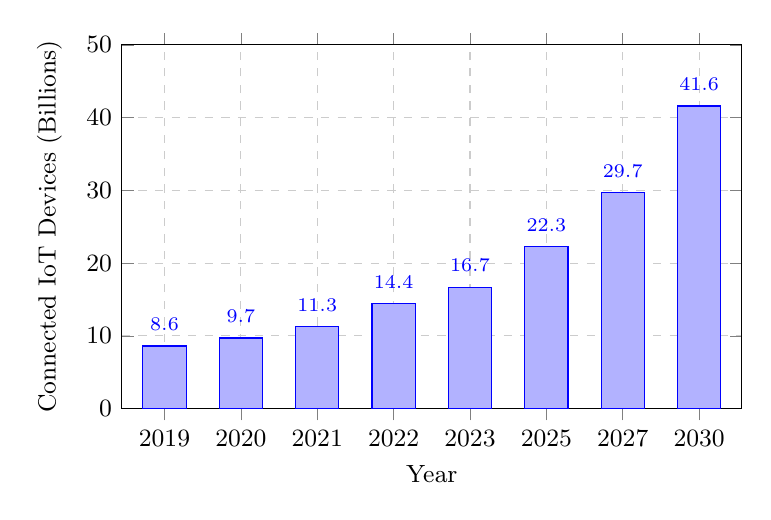
\begin{tikzpicture}
\begin{axis}[
  ybar,
  bar width     = 0.55cm,
  width         = 0.78\textwidth,
  height        = 6.2cm,
  xlabel        = {Year},
  ylabel        = {Connected IoT Devices (Billions)},
  xtick         = data,
  symbolic x coords = {2019,2020,2021,2022,2023,2025,2027,2030},
  xticklabel style  = {font=\small},
  yticklabel style  = {font=\small},
  xlabel style      = {font=\small},
  ylabel style      = {font=\small, yshift=2pt},
  ymin=0, ymax=50,
  ytick          = {0,10,20,30,40,50},
  nodes near coords,
  nodes near coords style={font=\scriptsize, yshift=2pt},
  every axis plot/.append style={fill=gray!55, draw=black!60},
  grid=major,
  grid style={dashed, gray!40},
  enlarge x limits = 0.08,
]
\addplot coordinates {
  (2019,8.6)
  (2020,9.7)
  (2021,11.3)
  (2022,14.4)
  (2023,16.7)
  (2025,22.3)
  (2027,29.7)
  (2030,41.6)
};
\end{axis}
\end{tikzpicture}
\caption{Growth of global connected IoT devices (2019--2030).
         Values for 2025--2030 are projections
         (Sources: IoT Analytics, Statista, IDC).}
\label{fig:iot_growth}
\end{figure}

As Figure~\ref{fig:iot_growth} illustrates, the global IoT device
count is projected to exceed 41 billion by 2030~\cite{iotanalytics2023},
driving the edge computing market toward USD 232 billion at a 25\%
compound annual growth rate~\cite{grandview2024edge}. IDC estimates
that 75\% of enterprise data will be processed outside the cloud by
2025~\cite{idc2020data}. This scale makes efficient resource
management at the edge not a convenience but a necessity.

Mobile Edge Computing (MEC) addresses the latency problem by placing
compute resources---cloudlets or edge servers---at the network
periphery. However, edge cloudlets are resource-constrained: limited
CPU, restricted RAM, and finite queue lengths mean that congestion
under simultaneous task arrivals directly causes delays and drops.
How incoming tasks are distributed across these nodes---the load
balancing problem---determines whether the QoS promises of MEC are
actually delivered.

Conventional strategies such as Round Robin, Least Connection, and
the LBRO heuristic~\cite{nayyer2022lbro} are reactive: they act on
the current observed state but cannot anticipate near-future
congestion. Deep Reinforcement Learning (DRL) offers a better
alternative---an agent that learns a placement policy through
interaction, discovering strategies that jointly minimise latency,
drops, energy, and load imbalance. Augmenting the agent's state with
short-horizon forecasts from a GRU-LSTM predictor further allows
proactive routing away from cloudlets trending toward saturation.
This thesis proposes \textbf{DRL-LSTM-LBRO}, which integrates both
ideas into a single, end-to-end trained scheduling framework.

\section{Problem Statement}
\label{sec:problem}

Consider a MEC environment consisting of $N$ heterogeneous edge
cloudlets and a cloud fallback, each serving a stream of IoT tasks
with varying CPU and RAM demands. At every discrete time step, a new
task arrives and must be assigned to one of the available destinations
before the next time step. Each cloudlet operates as an M/M/$c$ queue
with a finite buffer; a task that arrives when the buffer is full is
dropped and incurs a penalty. Once accepted, a task's end-to-end
latency comprises propagation delay, queueing delay (governed by the
Erlang-C formula), and service time. The cloud is modelled as an
infinite-capacity fallback with a fixed Wide Area Network (WAN)
transmission delay.

The objective is to learn a task placement policy $\pi$ that maps the
observed system state $s_t$ to a placement action $a_t \in
\{0, 1, \ldots, N\}$ (where action $N$ denotes the cloud) such that
the following quantities are jointly minimised over the long run:

\begin{itemize}
  \item the fraction of tasks dropped due to queue overflow,
  \item the average end-to-end latency of completed tasks,
  \item the average energy consumed per task execution,
  \item the degree of load imbalance across the $N$ cloudlets.
\end{itemize}

These objectives are in partial tension with one another. Sending all
tasks to the most powerful cloudlet minimises latency for each
individual task but quickly saturates that node, leading to drops and
imbalance. Distributing work uniformly ignores node heterogeneity and
the varying resource demands of individual tasks. Learning a policy
that navigates these trade-offs---especially under non-stationary
workloads---is the central challenge addressed in this thesis.

\section{Research Objectives}
\label{sec:objectives}

The research objectives that guide this work are as follows:

\begin{enumerate}

  \item \textbf{Design a predictive state representation.}
  Develop a per-cloudlet GRU-LSTM load forecaster that estimates
  near-future CPU and RAM utilisation from a sliding window of recent
  observations, and incorporate these predictions into the state
  vector seen by the scheduling agent.

  \item \textbf{Formulate a multi-objective reward function.}
  Design a reward signal that simultaneously penalises task drops,
  deadline violations, excess latency, energy consumption, and load
  imbalance, and that includes mechanisms to prevent the
  policy-collapse failure mode observed in prior DRL schedulers.

  \item \textbf{Train and evaluate a DDQN scheduling agent.}
  Implement a Double DQN agent with experience replay and a target
  network, train it on a simulated MEC environment parameterised with
  real workload traces, and evaluate its performance against five
  published load balancing algorithms and a Proximal Policy
  Optimisation (PPO) baseline.

  \item \textbf{Quantify the contribution of LSTM-augmented state.}
  Conduct a controlled ablation study by training and evaluating a
  variant of the agent that receives no LSTM predictions, to isolate
  the contribution of load forecasting to overall system performance.

  \item \textbf{Assess scalability.}
  Extend the trained framework to a six-cloudlet topology without
  modifying the underlying architecture, and verify that the
  performance gains observed in the three-cloudlet baseline
  generalise to this larger setting.

\end{enumerate}

\section{Contributions of the Thesis}
\label{sec:contributions}

This thesis makes the following original contributions to the field of
intelligent task scheduling for IoT edge computing:

\begin{enumerate}

  \item \textbf{A two-stage predictive scheduling framework.}
  DRL-LSTM-LBRO integrates per-cloudlet GRU-LSTM load forecasting
  directly into the state space of a DDQN agent. Unlike prior
  approaches that treat forecasting and scheduling as separate
  components, the predicted load values are part of the observation
  the agent receives at every decision step, allowing the policy to
  reason about both the current and near-future system state.

  \item \textbf{A multi-objective reward with collapse prevention.}
  The reward function jointly optimises six criteria---latency,
  energy, task drop rate, deadline adherence, load imbalance, and
  overload prevention---through a weighted combination. The inclusion
  of explicit imbalance and overload penalties prevents the known
  failure mode in which a DRL agent concentrates all traffic on the
  strongest node, a behaviour that degrades fairness and accelerates
  saturation under variable load.

  \item \textbf{Comprehensive empirical evaluation.}
  The framework is evaluated against five published load balancing
  algorithms (LBRO~\cite{nayyer2022lbro},
  DeepRM~\cite{mao2016resource}, DRL-EdgeLB~\cite{liu2022edgelb},
  MADRL-MEC~\cite{zhao2022madrl}, Pred-LB~\cite{predlb2025}) and a
  PPO baseline~\cite{schulman2017ppo}, across 500 evaluation episodes
  (ten random seeds). Task workload parameters are derived from the
  Google Borg cluster trace to ensure realistic demand distributions.

  \item \textbf{Demonstrated scalability.}
  Without any modification to the network architecture or training
  procedure, DRL-LSTM-LBRO is retrained on a six-cloudlet topology
  and shown to maintain its advantage over classical and learning-based
  baselines, confirming that the framework is not tailored to a
  specific cloudlet count.

\end{enumerate}

\section{Organisation of the Thesis}
\label{sec:organisation}

The remainder of this thesis is structured as follows.

\textbf{Chapter~\ref{chap:lit}} surveys related work on load balancing
in edge computing, covering heuristic approaches, classical machine
learning methods, DRL-based schedulers, and predictive scheduling
techniques. It identifies the specific gaps that motivate the proposed
framework.

\textbf{Chapter~\ref{chap:methodology}} presents the system model
and the DRL-LSTM-LBRO framework. It defines the three-tier
IoT--edge--cloud architecture, the M/M/$c$ queuing model, and the
MDP formulation of the scheduling problem. It then describes the
GRU-LSTM load forecaster, the state and action space design, the
multi-objective reward function, and the Double DQN agent architecture
and training procedure.

\textbf{Chapter~\ref{chap:results}} presents the experimental setup,
the baseline algorithms, training convergence behaviour, the main
comparative results, the ablation study, the PPO comparison, and the
six-cloudlet scalability experiment. Each set of results is followed
by a focused discussion.

\textbf{Chapter~\ref{chap:conclusion}} summarises the key findings,
discusses the limitations of the current work, and outlines directions
for future research.
